\chapter{Fundamentals}
\label{chp:funda}
This chapter defines and illustrates terms required to understand this paper.

\section{Rectified Linear Unit}
The \ac{ReLU} is a commonly used activation function. Given an input $X$, \ac{ReLU} is defined by Equation \eqref{eq:relu}. \autocite{ElAmir.2020}
\begin{equation}
	\label{eq:relu}
	relu(X) = max(0,X)
\end{equation}

\section{Swish Activation Function}
The swish activation function $swish$ is defined by Equation \eqref{eq:swish}. \autocites{Ramachandran.2017}{Elfwing.2018}
\begin{equation}
\label{eq:swish}
\begin{array}{lcl}
	swish(x) & = & x \cdot sigmoid(x)\\
	sigmoid(x) & = &  \frac{1}{ 1+e^{-x}}
\end{array}
\end{equation}

\section{Categorical Cross Entropy Loss Function}
Given the predicted output $\hat{y}$ and the desired output $y$, the categorical cross entropy loss function $\mathcal{L}$ is defined by Equation \eqref{eq:entropy}. \autocites{ElAmir.2020}
\begin{equation}
\label{eq:entropy}
\mathcal{L}(y, \hat{y}) = \sum_{j}^{m} \sum_{y}^{n} (y_{ij} \cdot log(\hat{y}_{ji}))
\end{equation}

\section{Array}
An array is a finite, ordered list of similar objects. These objects can be arrays themselves. An array nested inside another array is called subarray. All subarrays inside an array have the same structure. Accordingly, an array can be seen as ordered, finite, nested lists of objects. The objects are accessed by their position in the list called index. The index ranges from $0$ to size$-1$. The size is the number of objects inside the array. Accessing an object is denoted by square brackets. For example, the object $a[2]$ at index $2$ in the array $a = [a,b,c,d]$ is $c$.\autocites{Black.2016}{Garcia.2005}
Another way to denote accessing an object of a multidimensional array is to separate the indices of different dimensions by a comma. Given a multidimensional array $a$, an object at the indices $i_1, i_2, \dots, i_n$ is denoted $a[i_1, i_2, \dots, i_n]$
with $i_d$ being the index in the $d$th dimension, $n \in [1;D]$, and $D$ being the number of dimensions of $a$. For example, given the array~$a$ of Table \ref{tab:array}, the object $a[0,0] = a[0][0]$ is $[1,2,3]$. \autocite{Castro.2010}
\par
An array can be described by its dimensionality and shape.
The dimensionality or number of dimensions is the nesting depth of an array.
The shape of an array is denoted by its size $\times$ the shape of its subarrays. If the array contains no subarrays its shape is denoted by its size. Thus, the product of all sizes in the shape is the total number of objects contained in an array.\autocites{Black.2016}{Garcia.2005} This is illustrated in Table \ref{tab:array}.
\begin{xltabular}{\textwidth}{cccc}\toprule
	\caption{Array} \label{tab:array}\\
	\textbf{Array} & \textbf{Contents} & \textbf{Shape} & \textbf{Dimensionality} \\\midrule \endhead
	$a$ & $
	\begin{bmatrix}
	\begin{bmatrix}
	\begin{bmatrix}
	1 & 2 & 3
	\end{bmatrix}\\
	\begin{bmatrix}
	4 & 5 & 6
	\end{bmatrix}\\
	\begin{bmatrix}
	7 & 8 & 9
	\end{bmatrix}	
	\end{bmatrix} &
	\begin{bmatrix}
	\begin{bmatrix}
	1 & 2 & 3
	\end{bmatrix}\\
	\begin{bmatrix}
	4 & 5 & 6
	\end{bmatrix}\\
	\begin{bmatrix}
	7 & 8 & 9
	\end{bmatrix}	
	\end{bmatrix} &
	\begin{bmatrix}
	\begin{bmatrix}
	1 & 2 & 3
	\end{bmatrix}\\
	\begin{bmatrix}
	4 & 5 & 6
	\end{bmatrix}\\
	\begin{bmatrix}
	7 & 8 & 9
	\end{bmatrix}	
	\end{bmatrix}
	\end{bmatrix}
	$ & $3 \times 3 \times 3$ & $3$\\\midrule
	$a[0]$ & $
	\begin{bmatrix}
	\begin{bmatrix}
	1 & 2 & 3
	\end{bmatrix}\\
	\begin{bmatrix}
	4 & 5 & 6
	\end{bmatrix}\\
	\begin{bmatrix}
	7 & 8 & 9
	\end{bmatrix}	
	\end{bmatrix}
	$ & $3 \times 3$ & $2$\\\midrule
	$a[0][0]$ & $
	\begin{bmatrix}
	1 & 2 & 3
	\end{bmatrix}
	$ & $3$ & $1$
	\\\bottomrule
\end{xltabular}


\par
In this paper, an array is used to generalize matrices and vectors for an arbitrary number of dimensions. 
A vector~$\vec{v}$ is seen as a one-dimensional array~$v$ with each scalar $\vec{v}_i$ being the object $v[i]$ with index~$i$.
A matrix $A$ is seen as a two-dimensional array $a$ with each scalar $A_{ij}$ being the object~$a[i][j]$ with row index~$i$ and column index~$j$.
\subsection{Array Visualization}
In the context of a \ac{CNN}, sometimes arrays are visualized. \autocites{Singh.2020}{ElAmir.2020}
In this paper, a three-dimensional array with shape $w \times h \times d$ is visualized as a cuboid of width $w$, height $h$, and depth $d$.
A two-dimensional array with shape~$w \times h$ is visualized as a cuboid or rectangle of width~$w$, height~$h$, and depth~$1$.
A one-dimensional array with shape~$w$ is visualized as cuboid or rectangle of width~$w$, height~$1$, and depth~$1$. \autocites{Ertel.2016}{Rawat.2017}{Sabour.2017}{Krizhevsky.2012}{LeCun.2015b}
This is illustrated in Figure \ref{fig:array}.
\begin{figure}[H]
	%\cube{x offset}{y offset}{width}{height}{depth}{color}{fillcolor}

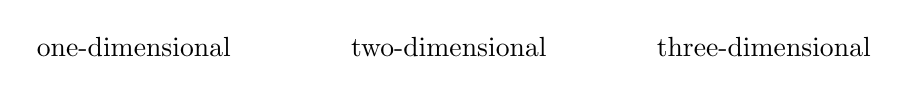
\begin{tikzpicture}[
cell/.style={
	rectangle, 
	rounded corners=2mm, 
	draw,
	very thick,
	align=center,
},
ArrowC1/.style={% Arrows with rounded corners
	rounded corners=.25cm,
	thick,
},
]
\cube{0}{0}{3}{3}{3}{black}{gray}
\cube{-4}{0}{3}{3}{1}{black}{gray}
\cube{-8}{-2}{3}{1}{1}{black}{gray}

\node (3d) at (-1.5,-4,0) {three-dimensional};
\node (2d) at (-5.5,-4,0) {two-dimensional};
\node (1d) at (-9.5,-4,0) {one-dimensional};

\end{tikzpicture}
	\caption{Array Visualization (own figure)}
	\label{fig:array}
\end{figure}
\subsection{Array Slice}
Given an array $a$, an array slice is denoted $a[start:end]$. $a[start:end]$ is defined as $a$ containing only the objects with indices in the range of $start$ to $end-1$. For example, given an array $a=[0,1,2,3,4,5]$, the array slice $a[1:3]$ is $[1,2]$. \autocite{Castro.2010}

\section{Machine Learning}
\label{sec:ml}
Machine learning in general is the art of training an algorithm to generate new information from data. The goal of machine learning is not to model explicitly how to extract this information, but to let the computer itself learn the model. \autocite{Mohri.2012} Machine learning has three main approaches: \autocite{ElAmir.2020}
\begin{itemize}
	\item Supervised learning \autocite{ElAmir.2020}
	\item Unsupervised learning \autocite{ElAmir.2020}
	\item Semi-supervised learning \autocite{ElAmir.2020}
\end{itemize}
As stated in Section \ref{sec:scope}, this paper is focused exclusively on supervised learning.

\subsection{Supervised Learning}
Supervised learning is the art of training an algorithm to generate new information from data samples and associated target outputs. The target outputs can consist of numeric values or string labels. String labels can be classes or tags. The goal of supervised learning is to learn a model that can predict the correct outputs when posed with new samples. Supervised learning approaches two problems: \autocite{ElAmir.2020}
\begin{itemize}
	\item Classification \autocite{ElAmir.2020}
	\item Regression \autocite{ElAmir.2020}
\end{itemize}
As stated in Section \ref{sec:scope}, this paper is focused exclusively on classification.

\subsection{Classification}
Classification is the problem of assigning the correct output classes to samples. For image classification, the samples are images. For \ac{CNN}s, an image is represented as a multidimensional array. \autocites{ElAmir.2020}{LeCun.2015b} The output is computed using the $softmax$ function. The $softmax$ function computes the probabilities of each target class over all  possible $c$~target classes. The predicted target class is the class with the highest probability. The $softmax$ function is defined by Equation \eqref{eq:softmax}.\autocite{ElAmir.2020}
\begin{equation}
	\label{eq:softmax}
	softmax(x) = \frac{e^x}{\sum_{i=0}^{c} e^{x_i}}
\end{equation}

\section{Neural Network}
\label{sec:neuralnetwork}
A neural network is a machine learning model and can be seen as a universal function approximator. A function approximator approximates a function. This function maps an input $X$ to an output $Y$.\autocites{Hornik.1989}{Ertel.2016}
In consequence, a neural network itself can be seen as a function. 
A neural network is structured in layers. \autocite{Ertel.2016}  A layer receives an input and returns an output. The first layer is called input layer, the last layer is called output layer, and the remaining layers are called hidden layers. \autocite{LeCun.2015b} A hidden layer is a layer which receives the output of its previous layer or previous layers as input. The input layer is the layer receiving the input of the neural network. The output layer is the layer returning the output of the neural network. This is illustrated in Figure~\ref{img:neuralnetwork}.
This way, layers themselves can be seen as functions. Hence, a neural network can be described as a chain of layer functions. Given the layer~$F_l$ at position~$l$, the input~$X$, and the output~$Y$ of the neural network~$F$, then $Y$ is computed as defined by Equation~\eqref{eq:neuralnetwork}.
\begin{equation}
	\label{eq:neuralnetwork}
	Y = F(X) = F_l(F_{l-1}\dots(F_1(X)\dots)) 
\end{equation}
\begin{figure}[H]
	\centering
	A neural network is a machine learning model and can be seen as a universal function approximator. A function approximator approximates a function. This function maps an input $X$ to an output $Y$.\autocites{Hornik.1989}{Ertel.2016}
In consequence, a neural network itself can be seen as a function. 
A neural network is structured in layers. \autocite{Ertel.2016}  A layer receives an input and returns an output. The first layer is called input layer, the last layer is called output layer, and the remaining layers are called hidden layers. \autocite{LeCun.2015b} A hidden layer is a layer which receives the output of its previous layer or previous layers as input. The input layer is the layer receiving the input of the neural network. The output layer is the layer returning the output of the neural network. This is illustrated in Figure~\ref{img:neuralnetwork}.
This way, layers themselves can be seen as functions. Hence, a neural network can be described as a chain of layer functions. Given the layer~$F_l$ at position~$l$, the input~$X$, and the output~$Y$ of the neural network~$F$, then $Y$ is computed as defined by Equation~\eqref{eq:neuralnetwork}.
\begin{equation}
	\label{eq:neuralnetwork}
	Y = F(X) = F_l(F_{l-1}\dots(F_1(X)\dots)) 
\end{equation}
\begin{figure}[H]
	\centering
	A neural network is a machine learning model and can be seen as a universal function approximator. A function approximator approximates a function. This function maps an input $X$ to an output $Y$.\autocites{Hornik.1989}{Ertel.2016}
In consequence, a neural network itself can be seen as a function. 
A neural network is structured in layers. \autocite{Ertel.2016}  A layer receives an input and returns an output. The first layer is called input layer, the last layer is called output layer, and the remaining layers are called hidden layers. \autocite{LeCun.2015b} A hidden layer is a layer which receives the output of its previous layer or previous layers as input. The input layer is the layer receiving the input of the neural network. The output layer is the layer returning the output of the neural network. This is illustrated in Figure~\ref{img:neuralnetwork}.
This way, layers themselves can be seen as functions. Hence, a neural network can be described as a chain of layer functions. Given the layer~$F_l$ at position~$l$, the input~$X$, and the output~$Y$ of the neural network~$F$, then $Y$ is computed as defined by Equation~\eqref{eq:neuralnetwork}.
\begin{equation}
	\label{eq:neuralnetwork}
	Y = F(X) = F_l(F_{l-1}\dots(F_1(X)\dots)) 
\end{equation}
\begin{figure}[H]
	\centering
	\input{img/neuralnetwork}
	\caption{Neural Network (own figure)} \label{img:neuralnetwork}
\end{figure}
A layer consists of neurons. Neurons are the basic processing units of neural networks. A neuron consists of $n$ weighted connections $w_i, i \in [1;n]$, a sum function $\sum$, and an activation function $\varphi$, see Figure \ref{img:neuron}. Each connection is connected to an input of the neuron. The sum function sums the weighted inputs. The activation function transforms the sum. The result of the activation function is the output $y$ of the neuron. \autocite{Ertel.2016} Given an input $x$, $y$ is computed as defined by Equation \eqref{eq:neurn}.
\begin{equation}
	\label{eq:neurn}
	y = \varphi(\sum x \cdot w)
\end{equation}
\begin{figure}[H]
	\centering
	\input{img/neuron}
	\caption{Neuron (own figure)} \label{img:neuron}
\end{figure}

	\caption{Neural Network (own figure)} \label{img:neuralnetwork}
\end{figure}
A layer consists of neurons. Neurons are the basic processing units of neural networks. A neuron consists of $n$ weighted connections $w_i, i \in [1;n]$, a sum function $\sum$, and an activation function $\varphi$, see Figure \ref{img:neuron}. Each connection is connected to an input of the neuron. The sum function sums the weighted inputs. The activation function transforms the sum. The result of the activation function is the output $y$ of the neuron. \autocite{Ertel.2016} Given an input $x$, $y$ is computed as defined by Equation \eqref{eq:neurn}.
\begin{equation}
	\label{eq:neurn}
	y = \varphi(\sum x \cdot w)
\end{equation}
\begin{figure}[H]
	\centering
	\begin{tikzpicture}[
cell/.style={
	rectangle, 
	rounded corners=2mm, 
	draw,
	very thick,
	align=center,
},
ArrowC1/.style={% Arrows with rounded corners
	rounded corners=.25cm,
	thick,
},
]
	\node (x0) at (0,3) {$x_0$};
	\node (x1) at (0,2) {$x_1$};
	\node (..) at (0,1) {$\vdots$};
	\node (xn) at (0,0) {$x_n$};
	\node[draw, circle, minimum size=1cm] (sum) at (2,1.5) {$\sum$};
	\node[draw, circle, minimum size=1cm] (phi) at (4,1.5) {$\varphi$};
	\node (y) at (6,1.5) {$y$};
	\draw[-latex,ArrowC1] (x0) -- (sum) node[sloped,pos=.3,above] {$w_0$};
	\draw[-latex,ArrowC1] (x1) -- (sum) node[sloped,pos=.3,above] {$w_1$};
	\draw[-latex,ArrowC1] (xn) -- (sum) node[sloped,pos=.3,above] {$w_n$};
	\draw[-latex,ArrowC1] (sum) -- (phi);
	\draw[-latex,ArrowC1] (phi) -- (y);
	\node[draw,	ellipse, minimum height=2cm,minimum width=3cm, label=Neuron] (neuron) at (3,1.5) {};
	\end{tikzpicture}
	\caption{Neuron (own figure)} \label{img:neuron}
\end{figure}

	\caption{Neural Network (own figure)} \label{img:neuralnetwork}
\end{figure}
A layer consists of neurons. Neurons are the basic processing units of neural networks. A neuron consists of $n$ weighted connections $w_i, i \in [1;n]$, a sum function $\sum$, and an activation function $\varphi$, see Figure \ref{img:neuron}. Each connection is connected to an input of the neuron. The sum function sums the weighted inputs. The activation function transforms the sum. The result of the activation function is the output $y$ of the neuron. \autocite{Ertel.2016} Given an input $x$, $y$ is computed as defined by Equation \eqref{eq:neurn}.
\begin{equation}
	\label{eq:neurn}
	y = \varphi(\sum x \cdot w)
\end{equation}
\begin{figure}[H]
	\centering
	\begin{tikzpicture}[
cell/.style={
	rectangle, 
	rounded corners=2mm, 
	draw,
	very thick,
	align=center,
},
ArrowC1/.style={% Arrows with rounded corners
	rounded corners=.25cm,
	thick,
},
]
	\node (x0) at (0,3) {$x_0$};
	\node (x1) at (0,2) {$x_1$};
	\node (..) at (0,1) {$\vdots$};
	\node (xn) at (0,0) {$x_n$};
	\node[draw, circle, minimum size=1cm] (sum) at (2,1.5) {$\sum$};
	\node[draw, circle, minimum size=1cm] (phi) at (4,1.5) {$\varphi$};
	\node (y) at (6,1.5) {$y$};
	\draw[-latex,ArrowC1] (x0) -- (sum) node[sloped,pos=.3,above] {$w_0$};
	\draw[-latex,ArrowC1] (x1) -- (sum) node[sloped,pos=.3,above] {$w_1$};
	\draw[-latex,ArrowC1] (xn) -- (sum) node[sloped,pos=.3,above] {$w_n$};
	\draw[-latex,ArrowC1] (sum) -- (phi);
	\draw[-latex,ArrowC1] (phi) -- (y);
	\node[draw,	ellipse, minimum height=2cm,minimum width=3cm, label=Neuron] (neuron) at (3,1.5) {};
	\end{tikzpicture}
	\caption{Neuron (own figure)} \label{img:neuron}
\end{figure}


\section{Training Neural Networks}
\label{sec:training}
Recapitulating, a neural network can be seen as a universal function approximator.\autocite{Ertel.2016} A loss function is a metric that measures how well a neural network approximates a function. The resulting value is called loss $\mathcal{L}$ \autocite{ElAmir.2020}. For example, if a function classifying tool images is to be approximated, the loss function measures how well the neural network classifies the tool images.
\par
Neural networks are trained by reducing the loss. The loss is reduced by adapting the parameters $\theta$ of the neural network in such a way that $\mathcal{L}$ is minimized. To properly adjust $\theta$, backpropagation \autocite{Rumelhart.1986} is used to calculate a gradient vector $\nabla {\theta}$. This gradient indicates by which amount the error increases or decreases if $\theta$ is increased by a very small amount. The loss function in regard to $\theta$ can be seen as high-dimensional hilly landscape, with the negative gradient vector indicating the direction of the steepest descent in that landscape. The gradient is used to descend in that landscape to find a local or the global minimum. \autocite{LeCun.2015} Accordingly, training a neural network can be seen as solving an optimization problem. \autocite{ElAmir.2020}  

\section{Optimizer}
\label{sec:optimizer}
An optimizer is an algorithm solving an optimization problem. Optimizers used in the course of this paper are \ac{SGD} with momentum or Nesterov momentum and \ac{RMSProp}.
%
\ac{SGD} and \ac{RMSProp} are based on gradient descent. Gradient descent is an algorithm minimizing a loss function $\mathcal{L}(\theta)$ in regard to the parameters~$\theta$ of a neural network. The loss function is minimized by changing the parameters by the negative gradient of the loss function $\nabla_{\theta} \mathcal{L}(\theta)$ with regard to the parameters. Before changing the parameters, the gradient is scaled by the learning rate $\eta$. This is repeated until a local or the global minimum is reached. While descending the landscape, the learning rate can be imagined as the size of a step taken in that landscape. \autocite{Ruder.2016}
%
\ac{SGD} approximates the gradient $\nabla_{\theta} \mathcal{L}(\theta)$ for each sample or batches of samples. On that account, \ac{SGD} is much faster but causes the loss function to fluctuate. The fluctuation is decreased by increasing the batch size. The change of parameters is defined in Equation \eqref{eq:sgd}. \autocite{Ruder.2016}
\begin{equation}
	\label{eq:sgd}
	\theta = \theta - \eta \nabla_{\theta} \mathcal{L}(\theta)
\end{equation}
%
\ac{SGD} can be augmented with momentum or Nesterov momentum.
%
Momentum accelerates \ac{SGD} by adding a fraction $\gamma$ of the previous step's gradient $v_{t-1}$ to the current step's gradient. This way, the gradient is increased for dimensions whose previous gradients point into the same directions and reduced for dimensions whose previous gradients point into different directions. In consequence, a local or the global minimum is reached faster and fluctuation of the loss function is reduced.
Momentum can be imagined as pushing down and gaining speed while descending the landscape. The problem is that when the landscape slopes up again the speed will result in an ascendance in the landscape. The change of parameters is defined in Equation \eqref{eq:momentum}. \autocite{Ruder.2016}
\begin{equation}
	\label{eq:momentum}
	\begin{array}{lcl}
		\theta & = & \theta - v_t\\
		v_t & = & \gamma v_{t-1} + \eta \nabla_{\theta} \mathcal{L}(\theta)
	\end{array}
\end{equation}
%
Nesterov momentum accelerates \ac{SGD} while descending and decelerates \ac{SGD} before ascending. Nesterov momentum does so by adding a fraction $\gamma$ of the previous step's gradient to an approximation of the next step's gradient $\nabla_{\theta} \mathcal{L}(\theta - \gamma v_{t-1})$ instead of the currents step's gradient. Approximating the next step's gradient can be imagined as looking ahead. Therefore, Nesterov momentum can be imagined as pushing down and gaining speed while looking ahead to decelerate when the landscape is about to slope up. The change of parameters is defined in Equation \eqref{eq:nesterov}. \autocite{Ruder.2016}
\begin{equation}
	\label{eq:nesterov}
	\begin{array}{lcl}
		\theta & = & \theta - v_t\\
		v_t & = & \gamma v_{t-1} + \eta \nabla_{\theta} \mathcal{L}(\theta - \gamma v_{t-1})
	\end{array}
\end{equation}
%
\ac{RMSProp} decreases fluctuation of the loss function by adapting the learning rate for each parameter $\theta_i$. The gradient of the loss function with regard to the parameter~$\theta_i$ at step~$t$ is called $g_{t,i}$. The learning rate is adapted by dividing it by a root mean square variation~$RMS(g_t)$ of $g_t$. The root mean square variation is defined in Equation~\eqref{eq:rms}. \autocite{Ruder.2016}
\begin{equation}
	\label{eq:rms}
	RMS(g_t) = \sqrt{\gamma E[g^2]_{t-1} + (1-\gamma) g^2_t}
\end{equation}
Dividing the learning rate by the root mean square variation increases the learning rate for small gradients and decreases the learning rate for large gradients. Thus, fluctuation of the loss function is decreased. The change of parameters is defined in Equation \eqref{eq:rmsprop}. \autocite{Ruder.2016}
\begin{equation}
\label{eq:rmsprop}
	\theta_{t+1} = \theta_t - \frac{\eta}{RMS(g_t) + \epsilon} g_t
\end{equation}
The noise parameter $\epsilon$ is close to $0$. Adding $\epsilon$ ensures that $\eta$ is never divided by zero. \autocite{Ruder.2016}
Note that some papers refer to the fraction $\gamma$ as momentum. \autocites{Simonyan.2014}{He.2016}{Xie.2017}{Huang.2017}{Tan.2019}

\section{Layers}
\label{sec:layers}
This section lists and explains basic layers used by neural networks described in this paper.
\subsection{Pooling}
A pooling function replaces the output at a certain location with a
summary statistic of the nearby outputs. \autocite{Goodfellow.2016} The following pooling functions are used by neural networks described in this paper.
\begin{itemize}
	\item Max Pooling
	\item Average Pooling
	\item Global Average Pooling
\end{itemize}
\subsubsection{Max Pooling}
The most widely used pooling technique is max pooling. Max pooling takes a maximum from all pools of input channels of the layer's input.\autocite{Singh.2020} The pools can be seen as array slices. These array slices are determined by pooling size $p$ and stride $stride$. The pooling size determines the shape of the pool. The pool is shaped $p \times p$. Stride is the number of rows and columns by which the pool is shifted to determine the next pool. This shifting can be imagined as sliding the pool over the input channel. Given an input channel $X$ with size $w \times h$, max pooling $maxpooling$ is defined as described by Equation \eqref{eq:pooling}. \autocite{Michelucci.2019}
\begin{equation}
	\label{eq:pooling}
	\begin{array}{l}
	maxpooling = max(X[i:i+p, j:j+p]) |\\
	i \in \{x|x_0=0, x \le w-p, x_{n+1} = x_n+stride\},\\
	j \in \{x|x_0=0, x \le h-p, _{n+1} = x_n+stride\}
	\end{array}
\end{equation}
For a better understanding, an example of max pooling is illustrated in Figure \ref{fig:pooling}. The figure displays an example of max pooling an input channel of shape $4 \times 4$, with a stride of 2, and a pooling size of 2. The different pools are highlighted in different colors. The result of a pool is highlighted in the color of that pool.
\begin{figure}[H]
	\centering
	\begin{tikzpicture}
\matrix (mtr) [matrix of nodes,row sep=-\pgflinewidth, nodes={draw}]
{
	|[fill=orange!30]| 8 & |[fill=orange!30]| 2 & |[fill=green!30!black!30]| 5 & |[fill=green!30!black!30]| 4 \\
	|[fill=orange!30]| 1 & |[fill=orange!30]| 0 & |[fill=green!30!black!30]| 7 & |[fill=green!30!black!30]| 1 \\
	|[fill=blue!30]| 1 & |[fill=blue!30]| 2 & |[fill=yellow!30]| 3 & |[fill=yellow!30]| 0 \\
	|[fill=blue!30]| 0 & |[fill=blue!30]| 2 & |[fill=yellow!30]| 1 & |[fill=yellow!30]| 2 \\ 
};

\node [below= of mtr-2-3.south west] (lm) {Input Channel};

\matrix (mt) [matrix of nodes,row sep=-\pgflinewidth, nodes={draw}, right = 4em of mtr]
{
	 |[fill=orange!30]| 8 &  |[fill=green!30!black!30]| 7 \\
	 |[fill=blue!30]| 2 &  |[fill=yellow!30]| 3 \\
};

\node [below= of mt-1-2.south west] (m) {Output};

\end{tikzpicture}
	\caption{Max Pooling Illustration (own figure)}
	\label{fig:pooling}
\end{figure}
\subsubsection{Average Pooling}
Another pooling technique is average pooling. 
%
Average pooling is used by DenseNet-264\autocite{Huang.2017} which is described in this paper. 
%
Understanding this neural network requires understanding average pooling. Average pooling works exactly the same as max pooling except that it takes the average instead of the maximum. Given an input channel~$X$ with size $w \times h$, average pooling~$avgpooling$ is defined as described by Equation~\eqref{eq:avgpooling}. \autocite{Michelucci.2019}
\begin{equation}
	\label{eq:avgpooling}
	\begin{array}{lcl}
		avgpooling & = & average(X[i:i+p, j:j+p]) |\\
		average(X) & = & \frac{\sum X}{|X|} 
	\end{array}
\end{equation}
\subsubsection{Global Average Pooling}
Another pooling technique is global average pooling. 
%
Global average pooling is used by ResNet-152\autocite{He.2016}, ResNeXt-101\autocite{Xie.2017}, DenseNet-264\autocite{Huang.2017}, and EfficientNet-B7\autocite{Tan.2019} which are described in this paper.
%
Understanding these neural networks requires understanding global average pooling. Global average pooling takes the average of each input channel. The input is an array of input channels. The output is an array containing the averages. Given an array of $d$ input channels $X$, global average pooling $globalavgpooling$ is defined as described by Equation \eqref{eq:globalavgpool}. \autocite{Lin.2013}
\begin{equation}
	\label{eq:globalavgpool}
	\begin{array}{lcl}
		globalavgpooling(X) & = & concat(globalavgpooling_0, \dots, globalavgpooling_{d-1})\\
		globalavgpoolingg_i & = & average(X_i)\\
		average(X) & = & \frac{\sum X}{|X|} 
	\end{array}
\end{equation}
 

\subsection{Dense}
A dense layer is a layer in which each neuron is connected to each input of the layer, see Figure \ref{fig:dense}. Given the weights of the neurons $W$, an input $X$, and an activation function $\varphi$, the dense layer $dense$ is described by Equation \eqref{eq:dense}. \autocite{Singh.2020}
\begin{equation}
	\label{eq:dense}
	dense(X) = \varphi(X \cdot W)
\end{equation}
\begin{figure}[H]
	\centering
	Dense convolutional neural networks address a problem of deep \ac{CNN}s. \autocite{Huang.2017}
\blockquote[\cite{Huang.2017}]{As information about the input or gradient passes through many layers, it can vanish and \enquote{washout} by the time it reaches the end (or beginning) of the network.
}
Dense convolutional neural networks address this problem by connecting all layers with each other, see Figure \ref{fig:denseconv}. The input of a layer is the concatenation of the original input and all outputs of previous layers. This way, information flow between layers in the network is encouraged. \autocite{Huang.2017}
\begin{figure}[H]
	\centering
	
%\cube{x offset}{y offset}{width}{height}{depth}{color}{fillcolor}
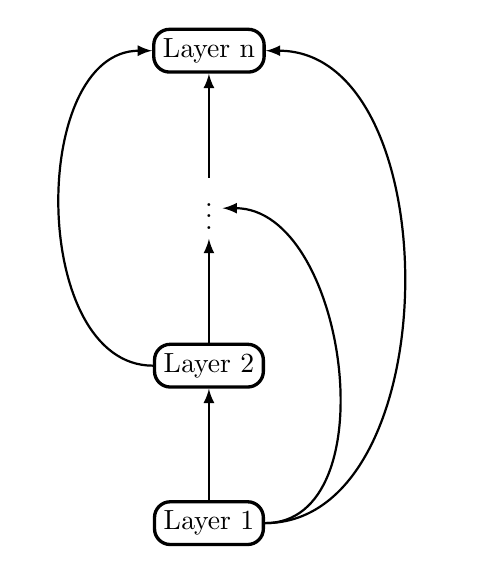
\begin{tikzpicture}[
	cell/.style={
		rectangle, 
		rounded corners=2mm, 
		draw,
		very thick,
		align=center,
	},
	ArrowC1/.style={% Arrows with rounded corners
		rounded corners=.25cm,
		thick,
	},
]

\node[cell] (l1) at (0,0) {Layer 1};
\node[cell] (l2) at (0,2) {Layer 2};
\node (dots) at (0,4) {$\vdots$};
\node[cell] (ln) at (0,6) {Layer n};

\draw[-latex, ArrowC1] (l1) -- (l2);
\draw[-latex, ArrowC1] (l2) -- (dots);
\draw[-latex, ArrowC1] (dots) -- (ln);

\draw[-latex, ArrowC1] (l1) to[out=0, in=0] (ln);
\draw[-latex, ArrowC1] (l1) to[out=0, in=0] (dots);

\draw[-latex, ArrowC1] (l2) to[out=-180, in=180] (ln);

	
\end{tikzpicture}
	\caption{Dense Convolutional Neural Network (own figure)}
	\label{fig:denseconv}
\end{figure}
\par
An additional, counter-intuitive effect of dense convolutional neural networks is that they require fewer parameters. 
Traditional neural networks pass information from layer to layer. Consequently, layers need to learn what information needs to be added and preserved. Dense convolutional neural networks explicitly distinguish between added and preserved information. Features are reused. Thus, they do not need to learn which information to preserve. Therefore, they need fewer parameters. \autocite{Huang.2017}
\par
The best-performing dense convolutional neural network found in the course of the literature review is the $264$ layer version of \cite{Huang.2017}'s DenseNet, called DenseNet-264.
The input of DenseNet-264 is a $224$-by-$224$-pixel, \ac{RGB} image. The output of DenseNet-264 comprises the probabilities of the $c$ target classes. 
DenseNet-264 is comprised of convolutional layers followed by $1$ dense layer. \autocite{Huang.2017}
\par
The convolutional layers have a stride of $1$ and a padding preserving spatial dimensions.
The first convolutional layer has $64$ kernels of size $7$ and a stride of $2$. It is followed by batch normalization, \ac{ReLU} activation function, and max pooling. Max pooling is applied with a pooling size of $3$, a pooling stride of $2$, and a padding preserving spatial dimensions. \autocite{Xie.2017}
The remaining convolutional layers are arranged in $4$ dense blocks and $3$ transition layers. A transition layer is applied between each dense block.
After the last dense block batch normalization, \ac{ReLU} activation function, global average pooling, and a dense layer are applied.
The dense layer has $c$ neurons and uses the softmax activation function. \autocite{Huang.2017}
\par
A dense block consists of $L$ convolutional blocks. All convolutional blocks are connected with each other. In consequence, the input of the $l$th convolutional block is the concatenation of the input of the dense block and the outputs of all previous layers. The output of the dense block is the concatenation of the input of the dense block and the outputs of all convolutional blocks of the dense block. Therefore, inside the dense block, the spatial dimensions of all feature maps are the same. A convolutional block consists of $2$~convolutional layers. The first layer has $128$~kernels of size~$1$. The second layer has $32$~kernels of size~$3$. Batch normalization and \ac{ReLU} activation function are applied before each convolution. The configurations of each dense block are outlined in Table \ref{tab:densenet}. \autocite{Huang.2017}
\par
A transition layer reduces the number and spatial dimensions of the feature maps.
A transition layer consists of the sequence batch normalization, \ac{ReLU} activation function, convolution, and average pooling. The convolution is used to reduce the number of feature maps by factor $0.5$. Hence, the convolution has $0.5 \cdot d$ kernels of size~$1$ with $d$ being the initial number of feature maps. The average pooling is used to reduce the spatial dimensions of the feature maps. The pooling is of size $2$ and has a stride~of~$2$. \autocite{Huang.2017}
\par
The whole configuration of DenseNet-264 is outlined in Table \ref{tab:densenet}. \autocite{Huang.2017}
\begin{xltabular}{\textwidth}{lX}\toprule
	\caption[DenseNet-264 Configuration]{DenseNet-264 Configuration. Note that each $k \times k \text{ conv } K$ denotes the sequence batch normalization, \ac{ReLU}, and convolution with $K$ kernels of size  $k$, except for the first $\text{conv}$, which denotes the sequence convolution, batch normalization \ac{ReLU}.} \label{tab:densenet}\\
	\textbf{Layer/Block} & \textbf{Configuration}\\\midrule \endhead
	Input Layer & $7 \times 7 \text{ conv } 64$, stride $2$, and $3 \times 3$ max pooling, stride $2$\\\midrule
	Dense Block $1$ & $\begin{bmatrix}
	1 \times 1 \text{ conv } 128\\
	3 \times 3 \text{ conv } 32
	\end{bmatrix} \times 6$\\\midrule
	Transition Layer $1$ & $1 \times 1 \text{ conv } 0.5d$, stride $2$, and $2 \times 2$ average pooling, stride $2$\\\midrule
	Dense Block $2$ & $\begin{bmatrix}
	1 \times 1 \text{ conv } 128\\
	3 \times 3 \text{ conv } 32
	\end{bmatrix} \times 12$\\\midrule
	Transition Layer $2$ & $1 \times 1 \text{ conv } 0.5d$, stride $2$, and $2 \times 2$ average pooling, stride $2$\\\midrule
	Dense Block $3$ & $\begin{bmatrix}
	1 \times 1 \text{ conv } 128\\
	3 \times 3 \text{ conv } 32
	\end{bmatrix} \times 64$\\\midrule
	Transition Layer $3$ & $1 \times 1 \text{ conv } 0.5d$, stride $2$, and $2 \times 2$ average pooling, stride $2$\\\midrule
	Dense Block $4$ & $\begin{bmatrix}
	1 \times 1 \text{ conv } 128\\
	3 \times 3 \text{ conv } 32
	\end{bmatrix} \times 48$\\\midrule
	Output Layer & batch normalization, \ac{ReLU}, global average pooling, and dense with $c$ neurons
	\\\bottomrule
\end{xltabular}
	\caption{Dense Layer (own figure)}
	\label{fig:dense}
\end{figure}


\subsection{Batch Normalization}
Batch normalization is a technique to speed up training. Training is sped up by smoothing the optimization landscape and stabilizing the gradients. \autocite{Santurkar.2018}
Batch normali\-zation normalizes an input by subtracting the mean and dividing by the standard deviation. Mean and standard deviation are approximated batch-wise. Computation over a batch is more efficient, but mean and standard deviation vary dependent on the batch. Therefore, the true mean and standard deviation are approximated over multiple batches by learnable parameters. Given a batch of $m$ inputs $\mathcal{B} = \{x_1, x_2, \dots, x_m \}$, learnable parameters $\gamma, \beta$, and a noise $\epsilon$, batch normalization $batchnorm$ is defined by Equation \eqref{eq:batchnorm}. \autocite{Ioffe.2015} Noise ensures that division by $0$ does not occur.
\begin{equation}
	\label{eq:batchnorm}
	\begin{array}{lcl}
		batchnorm(x) & = & \gamma \hat{x} + \beta \\
		\hat{x} & = & \frac{x-\mu}{\sqrt{\sigma^2+\epsilon}}\\
		\mu & = & \frac{1}{m} \sum_{i=1}^{m} b_i | b_i \in \mathcal{B}\\
		\sigma & = & \frac{1}{m} \sum_{i=1}^{m} (b_i-\mu)^2 | b_i \in \mathcal{B}\\
	\end{array}
\end{equation}

\subsection{Dropout}
Dropout is a regularization technique addressing the problem of overfitting. 
Dropout randomly drops neurons during training. Dropping means removing the neuron temporarily, along with its connections. The probability of a neuron being dropped is called dropout rate $q$. Neurons are only dropped during training. After training, each neuron is retained and their weights are scaled down by the probability of a neuron being retained $p=1-q$.\autocite{Srivastava.2014}





%\subsection{Flatten} brauchst du nicht? Weil def dens layer alle neurons zu allen connected ist da ist egal ob vector oder matrix oder 3d tensor